%%
%% MemoryLab (c) 2021-24 Christopher A. Bohn
%%
%% Licensed under the Apache License, Version 2.0 (the "License");
%% you may not use this file except in compliance with the License.
%% You may obtain a copy of the License at
%%     http://www.apache.org/licenses/LICENSE-2.0
%% Unless required by applicable law or agreed to in writing, software
%% distributed under the License is distributed on an "AS IS" BASIS,
%% WITHOUT WARRANTIES OR CONDITIONS OF ANY KIND, either express or implied.
%% See the License for the specific language governing permissions and
%% limitations under the License.
%%

%%
%% (c) 2021 Christopher A. Bohn
%%

\documentclass[12pt]{article}

\usepackage{fullpage}
\usepackage{fancyhdr}
\usepackage[procnames]{listings}
\usepackage{hyperref}
\usepackage{textcomp}
\usepackage{bold-extra}
\usepackage[dvipsnames]{xcolor}
\usepackage{etoolbox}


% Customize the semester (or quarter) and the course number

\newcommand{\courseterm}{Spring 2022}
\newcommand{\coursenumber}{CSCE 231}

% Customize how a typical lab will be managed;
% you can always use \renewcommand for one-offs

\newcommand{\runtimeenvironment}{your account on the \textit{csce.unl.edu} Linux server}
\newcommand{\filesource}{Canvas or {\footnotesize$\sim$}cse231 on \textit{csce.unl.edu}}
\newcommand{\filesubmission}{Canvas}

% These are placeholder commands and will be renewed in each lab

\newcommand{\labnumber}{}
\newcommand{\labname}{Lab \labnumber\ Assignment}
\newcommand{\shortlabname}{}
\newcommand{\duedate}{}

% Individual or team effort

\newcommand{\individualeffort}{This is an individual-effort project. You may discuss concepts and syntax with other students, but you may discuss solutions only with the professor and the TAs. Sharing code with or copying code from another student or the internet is prohibited.}
\newcommand{\teameffort}{This is a team-effort project. You may discuss concepts and syntax with other students, but you may discuss solutions only with your assigned partner(s), the professor, and the TAs. Sharing code with or copying code from a student who is not on your team, or from the internet, is prohibited.}
\newcommand{\freecollaboration}{In addition to the professor and the TAs, you may freely seek help on this assignment from other students.}
\newcommand{\collaborationrules}{}

% Do you care about software engineering?

\providebool{allowspaghetticode}

\setbool{allowspaghetticode}{false}

\newcommand{\softwareengineeringfrontmatter}{
    \ifboolexpe{not bool{allowspaghetticode}}{
        \section*{No Spaghetti Code Allowed}
        In the interest of keeping your code readable, you may \textit{not} use
        any \lstinline{goto} statements, nor may you use any \lstinline{break}
        statements to exit from a loop, nor may you have any functions
        \lstinline{return} from within a loop.
    }{}
}

\newcommand{\spaghetticodepenalties}[1]{
    \ifboolexpe{not bool{allowspaghetticode}}{
        \penaltyitem{1}{for each \lstinline{goto} statement, \lstinline{break}
            statement used to exit from a loop, or \lstinline{return} statement
            that occurs within a loop.}
    }{}
}

% You shouldn't need to customize these,
% but you can if you like

\lstset{language=C, tabsize=4, upquote=true, basicstyle=\ttfamily}
\newcommand{\function}[1]{\textbf{\lstinline{#1}}}
\setlength{\headsep}{0.7cm}
\hypersetup{colorlinks=true}

\newcommand{\startdocument}{
    \pagestyle{fancy}
    \fancyhf{}
    \lhead{\coursenumber}
    \chead{\ Lab \labnumber: \labname}
    \rhead{\courseterm}
    \cfoot{\shortlabname-\thepage}

	\begin{document}
	\title{\ Lab \labnumber}
	\author{\labname}
	\date{Due: \duedate}
	\maketitle

    \textit{\collaborationrules}
}

\newcommand{\rubricitem}[2]{\item[\underline{\hspace{1cm}} +#1] #2}
\newcommand{\bonusitem}[2]{\item[\underline{\hspace{1cm}} Bonus +#1] #2}
\newcommand{\penaltyitem}[2]{\item[\underline{\hspace{1cm}} -#1] #2}

%%
%% labs/common/semester.tex
%% (c) 2021-22 Christopher A. Bohn
%%
%% Licensed under the Apache License, Version 2.0 (the "License");
%% you may not use this file except in compliance with the License.
%% You may obtain a copy of the License at
%%     http://www.apache.org/licenses/LICENSE-2.0
%% Unless required by applicable law or agreed to in writing, software
%% distributed under the License is distributed on an "AS IS" BASIS,
%% WITHOUT WARRANTIES OR CONDITIONS OF ANY KIND, either express or implied.
%% See the License for the specific language governing permissions and
%% limitations under the License.
%%


% Customize the semester (or quarter) and the course number

\newcommand{\courseterm}{Fall 2022}
\newcommand{\coursenumber}{CSCE 231}

% Customize how a typical lab will be managed;
% you can always use \renewcommand for one-offs

\newcommand{\runtimeenvironment}{your account on the \textit{csce.unl.edu} Linux server}
\newcommand{\filesource}{Canvas or {\footnotesize$\sim$}cse231 on \textit{csce.unl.edu}}
\newcommand{\filesubmission}{Canvas}

% Customize for the I/O lab hardware

\newcommand{\developmentboard}{Arduino Nano}
%\newcommand{\serialprotocol}{SPI}
\newcommand{\serialprotocol}{I2C}
%\newcommand{\displaymodule}{MAX7219digits}
%\newcommand{\displaymodule}{MAX7219matrix}
\newcommand{\displaymodule}{LCD1602}

\setbool{usedisplayfont}{true}

\newcommand{\obtaininghardware}{
    The EE Shop has prepared ``class kits'' for CSCE 231; your class kit costs \$30.
    The EE Shop is located at 122 Scott Engineering Center and is open M-F 7am-4pm. You do not need an appointment.
    You may pay at the window with cash, with a personal check, or with your NCard.
    The EE shop does \textit{not} accept credit cards.
}

% Update to reflect the CS2 course(s) at your institute

\newcommand{\cstwo}{CSCE~156, RAIK~184H, or SOFT~161}

% Do you care about software engineering?

\setbool{allowspaghetticode}{false}

% Which assignments are you using this semester, and when are they due?

\newcommand{\pokerlabnumber}{1}
\newcommand{\pokerlabcollaboration}{
    Sections~\ref{sec:connecting}, \ref{sec:terminology}, \ref{sec:gettingstarted}, \ref{subsec:typesofpokerhands}, and~\ref{subsec:studythecode}: \freecollaboration
    Sections~\ref{sec:completingcard} and~\ref{subsec:completepoker}: \individualeffort
}
\newcommand{\pokerlabdue}{Week of August 29, before the start of your lab section}

\newcommand{\keyboardlabnumber}{2}
\newcommand{\keyboardlabcollaboration}{\individualeffort}
\newcommand{\keyboardlabdue}{Week of January 31, before the start of your lab section}

\newcommand{\pointerlabnumber}{3}
\newcommand{\pointerlabcollaboration}{\individualeffort}
\newcommand{\pointerlabdue}{Week of February 7, before the start of your lab section}

\newcommand{\integerlabnumber}{4}
\newcommand{\integerlabcollaboration}{\individualeffort}
\newcommand{\integerlabdue}{Week of February 14, before the start of your lab section}

\newcommand{\floatlabnumber}{5}
\newcommand{\floatlabcollaboration}{\individualeffort}
\newcommand{\floatlabdue}{soon}

\newcommand{\addressinglabnumber}{6}
\newcommand{\addressinglabcollaboration}{\individualeffort}
\newcommand{\addressinglabdue}{Week of February 28, before the start of your lab section}

%bomblab was 7
%attacklab was 8

\newcommand{\pollinglabnumber}{9}
\newcommand{\pollinglabcollaboration}{\individualeffort}
\newcommand{\pollinglabdue}{Week of April 11, before the start of your lab section}
\newcommand{\pollinglabenvironment}{your \developmentboard-based class hardware kit}

\newcommand{\ioprelabnumber}{\pollinglabnumber-prelab}
\newcommand{\ioprelabcollaboration}{\freecollaboration}
\newcommand{\ioprelabdue}{Before the start of your lab section on April 5 or 6}

\newcommand{\interruptlabnumber}{10}
\newcommand{\interruptlabcollaboration}{\individualeffort}
\newcommand{\interruptlabdue}{Week of April 18, before the start of your lab section}
\newcommand{\interruptlabenvironment}{your \developmentboard-based class hardware kit}

\newcommand{\capstonelab}{ComboLock}    % this will come into play when we generalize capstonelab
\newcommand{\capstonelabnumber}{11}
\newcommand{\capstonelabcollaboration}{\teameffort}
\newcommand{\capstonelabdue}{Week of May 2, Before the start of your lab section\footnote{See Piazza for the due dates of teams with students from different lab sections.}}
\newcommand{\capstonelabenvironment}{your \developmentboard-based class hardware kit}

\newcommand{\memorylabnumber}{12}
\newcommand{\memorylabcollaboration}{This is an individual-effort project. You may discuss the nature of memory technologies and of memory hierarchies with classmates, but you must draw your own conclusions.}
\newcommand{\memorylabdue}{Week of May 2, at the end of your lab section}
\newcommand{\memorylabenvironment}{your \developmentboard-based class hardware kit and your account on the \textit{csce.unl.edu} Linux server}

% Labs not used this semester

\newcommand{\concurrencylabnumber}{XX}
\newcommand{\concurrencylabcollaboration}{\individualeffort}
\newcommand{\concurrencylabdue}{not this semester}

\newcommand{\ssbcwarmupnumber}{XX}
\newcommand{\ssbcwarmupcollaboration}{\freecollaboration}
\newcommand{\ssbcwarmupdue}{not this semester}

\newcommand{\ssbcpollingnumber}{XX}
\newcommand{\ssbcpollingcollaboration}{\individualeffort}
\newcommand{\ssbcpollingdue}{not this semester}

\newcommand{\ssbcinterruptnumber}{XX}
\newcommand{\ssbcinterruptcollaboration}{\individualeffort}
\newcommand{\ssbcinterruptdue}{not this semester}


\usepackage{graphicx}

%%% StickyNote from https://tex.stackexchange.com/questions/159679/sticky-notes-image
\usepackage{xparse}
% \usepackage{fontspec}
% \setmainfont{Humor Sans}
\usepackage{tikz}
\usetikzlibrary{shadows}
\usepackage{lipsum}\usepackage{array,color,colortbl}
\usepackage{listings}
\usepackage{lstlangarm}
\definecolor{LightGreen}{rgb}{0.88,1,0.88}

\definecolor{myyellow}{RGB}{242,226,149}

\NewDocumentCommand\StickyNote{O{6cm}mO{6cm}}{%
\begin{tikzpicture}
\node[
drop shadow={
  shadow xshift=2pt,
  shadow yshift=-4pt
},
inner xsep=7pt,
fill=myyellow,
xslant=-0.1,
yslant=0.1,
inner ysep=10pt
] {\parbox[t][#1][c]{#3}{#2}};
\end{tikzpicture}%
}
%%%

\renewcommand{\labnumber}{\memorylabnumber}
\renewcommand{\labname}{Memory Measurement Lab}
\renewcommand{\shortlabname}{memorylab}
\renewcommand{\collaborationrules}{\memorylabcollaboration}
\renewcommand{\duedate}{\memorylabdue}
\newcommand{\nano}{\developmentboard} % TODO: replace \nano with \developmentboard
\renewcommand{\runtimeenvironment}{\memorylabenvironment}
\pagelayout
\begin{document}
\labidentifier


In this assignment, you will measure the speed of different memories and draw
conclusions based on your understanding of memory hierarchies. \textbf{You will
be able to complete this lab assignment during lab time.}

%The instructions are written assuming you will run the code on
%\runtimeenvironment.

\section*{Learning Objectives}

After successful completion of this assignment, students will be able to:
\begin{itemize}
\item Identify the relative speeds of some types of memory.
\item Draw conclusions about a cache's design based on timing data.
\item Recognize the performance benefits of cache-friendly code.
\end{itemize}


\section*{During Lab Time}

\textbf{You must complete this lab assignment during lab time}; it is due at the
end of your scheduled lab session. The TAs will be available to answer
questions.

\section{Scenario}

{\large \textbf{Mid-Credits Scene}:} Herb walks up to you. ``Could you do me a
favor, please? I'd like to better characterize some of the performance
characteristics of the Cow Pi, but I don't have the time to do so. Now that the
urgency over developing the security systems is behind us, I need to get back to
Eclectic Electronics to clean up a couple of messes that I had to leave there
while we developed the Cow Pi. Do you mind measuring the memory performance?''


\section{Getting Started}

\subsection{RP2040 Memories}

The Raspberry Pi Pico on your Cow~Pi has two memories:

\begin{itemize}
    \item 264KB SRAM data memory
    \item 2MB Flash instruction memory
%    \item SRAM Instruction cache (the size of which you will deduce in this assignment)
\end{itemize}

Unlike modern microprocessors, most microcontrollers don't have cache
memories because the CPU and memory speeds are well-matched.
For example, the RP2040 on a Raspberry Pi Pico is clocked at 133MHz, about one order of magnitude slower than the microprocessor in your personal computer.
It doesn't have a cache for the data memory, whose speed is well-matched,
but it does have a 2-way set associative cache for the instruction memory.
Because it shares the same address space as the data memory, we will be able to read from instruction memory to influence the cache's contents.

%The instruction memory is designed to deliver instructions quickly, given the
%predictable access pattern for instruction fetches. This allows the CPU in the
%ATmega328P to have a 2-stage pipeline, as shown in Figure~\ref{fig:pipelining}.
%It is possible to place read-only data in the flash
%memory;\footnote{\url{https://www.nongnu.org/avr-libc/user-manual/pgmspace.html}}$^,$\footnote{\url{https://www.nongnu.org/avr-libc/user-manual/pgmspace_8h.html}}
%however, random accesses to the flash memory will require more than the one
%clock cycle that instruction fetches enjoy. (Similarly, read-only data can be
%placed in the EEPROM,\footnote{\url{https://www.nongnu.org/avr-libc/user-manual/group__avr__eeprom.html}}
%but we will not measure the EEPROM's performance in this lab assignment.)
%
%\begin{figure}
%    \centering
%    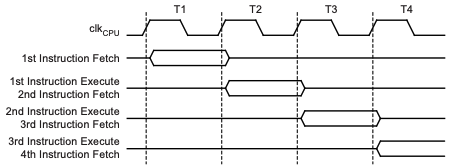
\includegraphics[width=10cm]{ATmega328P_PipelineTiming}
%    \caption{Pipelined instruction fetches and instruction executions. \tiny Copied from ATmega328P Data Sheet, Figure~6-4 \label{fig:pipelining}}
%\end{figure}


\subsection{Getting/Offering Help for Collecting Data}

If you forgot to bring your Cow~Pi to lab, or if you cannot establish a serial connection to the board (can you upload code from VS~Code by using the ``upload'' button?),
then you will need to work with someone else to collect data.
Students using Mac or Linux, and about half of the students using Windows, should be able to establish a serial connection.
\textit{You may work with another student to collect data, and you may discuss the nature of memory technologies and of memory hierarchies with other students, but \textbf{you must draw your own conclusions.}}

The program that you will use to take measurements sends its output to PlatformIO's serial monitor so that you can easily copy/paste its output into the \textit{CacheCharts.xlsx} spreadsheet.

The simulator that some students used for PollingLab and InterruptLab will not work for this assignment, because it does not simulate the flash memory's performance.
(It treats all accesses to the instruction memory as though they are cache hits, even when using a feature of the RP2040 that allows us to bypass the cache.)



\subsection{Start the Program}

The starter code, besides assorted header files and configuration files, consists of:
\begin{description}
    \item[MemoryLab.cpp] Driver code
    \item[memory\_measurement.c] Code to measure the speed of memory reads
    \item[cache\_measurement.c] Code to obtain data that will allow you to infer information about the RP2040's instruction cache
    \item[answers.txt] A text file with questions for you to answer
    \item[CacheCharts.xlsx] A spreadsheet that will parse the program's output to generate graphs
\end{description}

You do not need to (and should not) edit any files other than \textit{answers.txt} and \textit{CacheCharts.xlsx}.

\begin{description}
    \checkoffitem{Open the starter code in VS~Code as a PlatformIO project.}
    \checkoffitem{Open \textit{answers.txt}.}
    \checkoffitem{Open \textit{CacheCharts.xlsx}.}
    \checkoffitem{Connect your Cow~Pi to your laptop.}
    \checkoffitem{Open the PlatformIO Serial Monitor in VS~Code.}
    \checkoffitem{Compile the program and upload it to your Cow~Pi.}
\end{description}

The Serial Monitor will show:

\begin{verbatim}
  1. Measure SRAM and Flash memory access times
  2. Measure the size of the instruction cache using timing data
  3. Determine the size of a cache line using timing data
Please choose the measurement you wish to take:
\end{verbatim}

%\begin{verbatim}
%  1. Measure SRAM and Flash memory access times
%  2. Measure the size of the instruction cache using timing data
%  3. Determine the size of a cache line using timing data
%  4. Determine the size of a cache line using hit rate
%Please choose the measurement you wish to take:
%\end{verbatim}

When you make your selections, use your laptop's keyboard.
You will not need to press the Return key.


\section{Measuring Memory Speed}

In \textit{memory\_measurement.c} you'll find three functions,
\function{time_register_access()}, \function{time_sram_access()}, and \function{time_flash_access()}.
Each of functions repeatedly adds a value to a variable.
In \function{time_register_access()}, the values are in registers:

\begin{lstlisting}[language=c]
    start = get_microseconds();
    sum += a0;
    sum += a1;
    sum += a2;
    sum += a3;
    stop = get_microseconds();
    register_access_time += (stop - start);
\end{lstlisting}

compiles to

\begin{lstlisting}[language={[ARM]Assembler}]
    bl      get_microseconds
    movs    r5, r0
    add     r4, r4, r10
    add     r4, r4, r9
    add     r4, r4, r8
    adds    r4, r4, r7
    bl      get_microseconds
\end{lstlisting}

In the \function{time_sram_access()} and \function{time_flash_access()} functions, the values are in memory:

\begin{lstlisting}[language=c]
    unsigned long volatile *p = array + j;
    start = get_microseconds();
    sum += *p;
    sum += *(p + 8);
    sum += *(p + 16);
    sum += *(p + 24);
    stop = get_microseconds();
    sram_access_time += (stop - start);
\end{lstlisting}

compiles to

\begin{lstlisting}[language={[ARM]Assembler}]
    bl      get_microseconds
    movs    r6, r0
    ldr     r3, [r4]
    adds    r3, r7, r3
    ldr     r2, [r4, #32]
    adds    r3, r3, r2
    ldr     r2, [r4, #64]
    adds    r3, r3, r2
    ldr     r7, [r4, #96]
    adds    r7, r3, r7
    bl      get_microseconds
\end{lstlisting}

Thus, by subtracting the execution time for a function whose values are in memory from the execution time for the function whose values are in registers,
we will have the amount of time spent loading values from memory.
In \function{time_sram_access()}, the array is at an arbitrary location in data memory.
In \function{time_flash_access()}, the array is at one of the addresses that map to the flash instruction memory; its particular address is one that bypasses the cache and will always read directly from the flash memory.

\begin{description}
    \checkoffitem{Using your laptop's cursor in the Serial Monitor, press your laptop's \textbf{1} key (\textit{Measure SRAM and Flash memory access times}).}
    \checkoffitem{Answer questions 1--6 in \textit{answers.txt}.}
\end{description}

\begin{enumerate}
    \item What is the microcontroller's clock period, in microseconds?

        The RP2040's clock frequency is 133MHz, or 133 megacycles per second.
        You can determine its period, in microseconds, by dividing $\frac{1}{133}$.

    \item What is the reported time required to access data in SRAM?

        Copy the value from the output in the Serial Monitor.

    \item Is the reported time required to access data in SRAM consistent with
        information in the Cortex-M0+ Technical Reference Manual?
        Explain why or why not.

        The \href{https://developer.arm.com/documentation/ddi0484/c/Programmers-Model/Instruction-set-summary}{Instruction Set Summary in ARM's Cortex-M0+ Technical Reference Manual}
        states that the \lstinline{ldr} instruction will take two clock cycles to read from SRAM\@.

    \item What is the reported time required to access data in flash memory?

        Copy the value from the output in the Serial Monitor.

    \item How many clock cycles are required to access data in flash memory?

        Do the math.

    \item What can you conclude about the relative speeds of SRAM and flash memory?

        Is the difference important?
        Is the instruction cache necessary, or is it just ``nice to have''?
        Justify your conclusion with the data you collected.

\end{enumerate}


\section{Measuring the Size of the Cache}

One of the functions in \textit{cache\_measurement.c} is \function{measure_cache_size()}.
This function, with the assistance of a helper function, iterates over an ``array'' that  is at one of the addresses that map to the flash instruction memory;
its particular address is one that uses the cache.
On a cache hit, the value is read from the cache's SRAM;
on a cache miss, the value is retrieved from flash memory, and the corresponding block is placed in the cache.

While the first access to the array's elements will probably be misses,
by repeatedly reading from the array, we expect that most accesses will be hits.
Until the size of the ``array'' is too great to fit into the cache, that is.
When that happens, we will thrash the cache, causing all (or nearly all) accesses to be misses.

The \function{measure_cache_size()} will increase the size of the ``array'' until it is too great to fit into the cache.
The program will measure how much CPU time your process spends accessing the data.
We are less concerned with the specific amount of time, as we are with when the program stops being ``fast.''
(This is a subjective inference, but the data you collect from the RP2040 for this part of the lab won't be subtle.)

Figure~\ref{fig:LaptopCache} shows a graph similar to the one you will produce.
The figure shows the cache size measurements for an Intel Core i7 processor in a 2018 MacBook Pro.
This particular processor has a 32KB L1 data cache (also a 32KB L1 instruction cache), a 256KB L2 cache, and a 2MB L3 cache.
There are labels showing where these limits are exceeded -- other measurement artifacts make it difficult to discern the limit of the L1 cache, but we can use the chart to reasonably estimate the sizes of the L2 and L3 caches with an error less than a factor of 2.

\begin{figure}
    \centering
    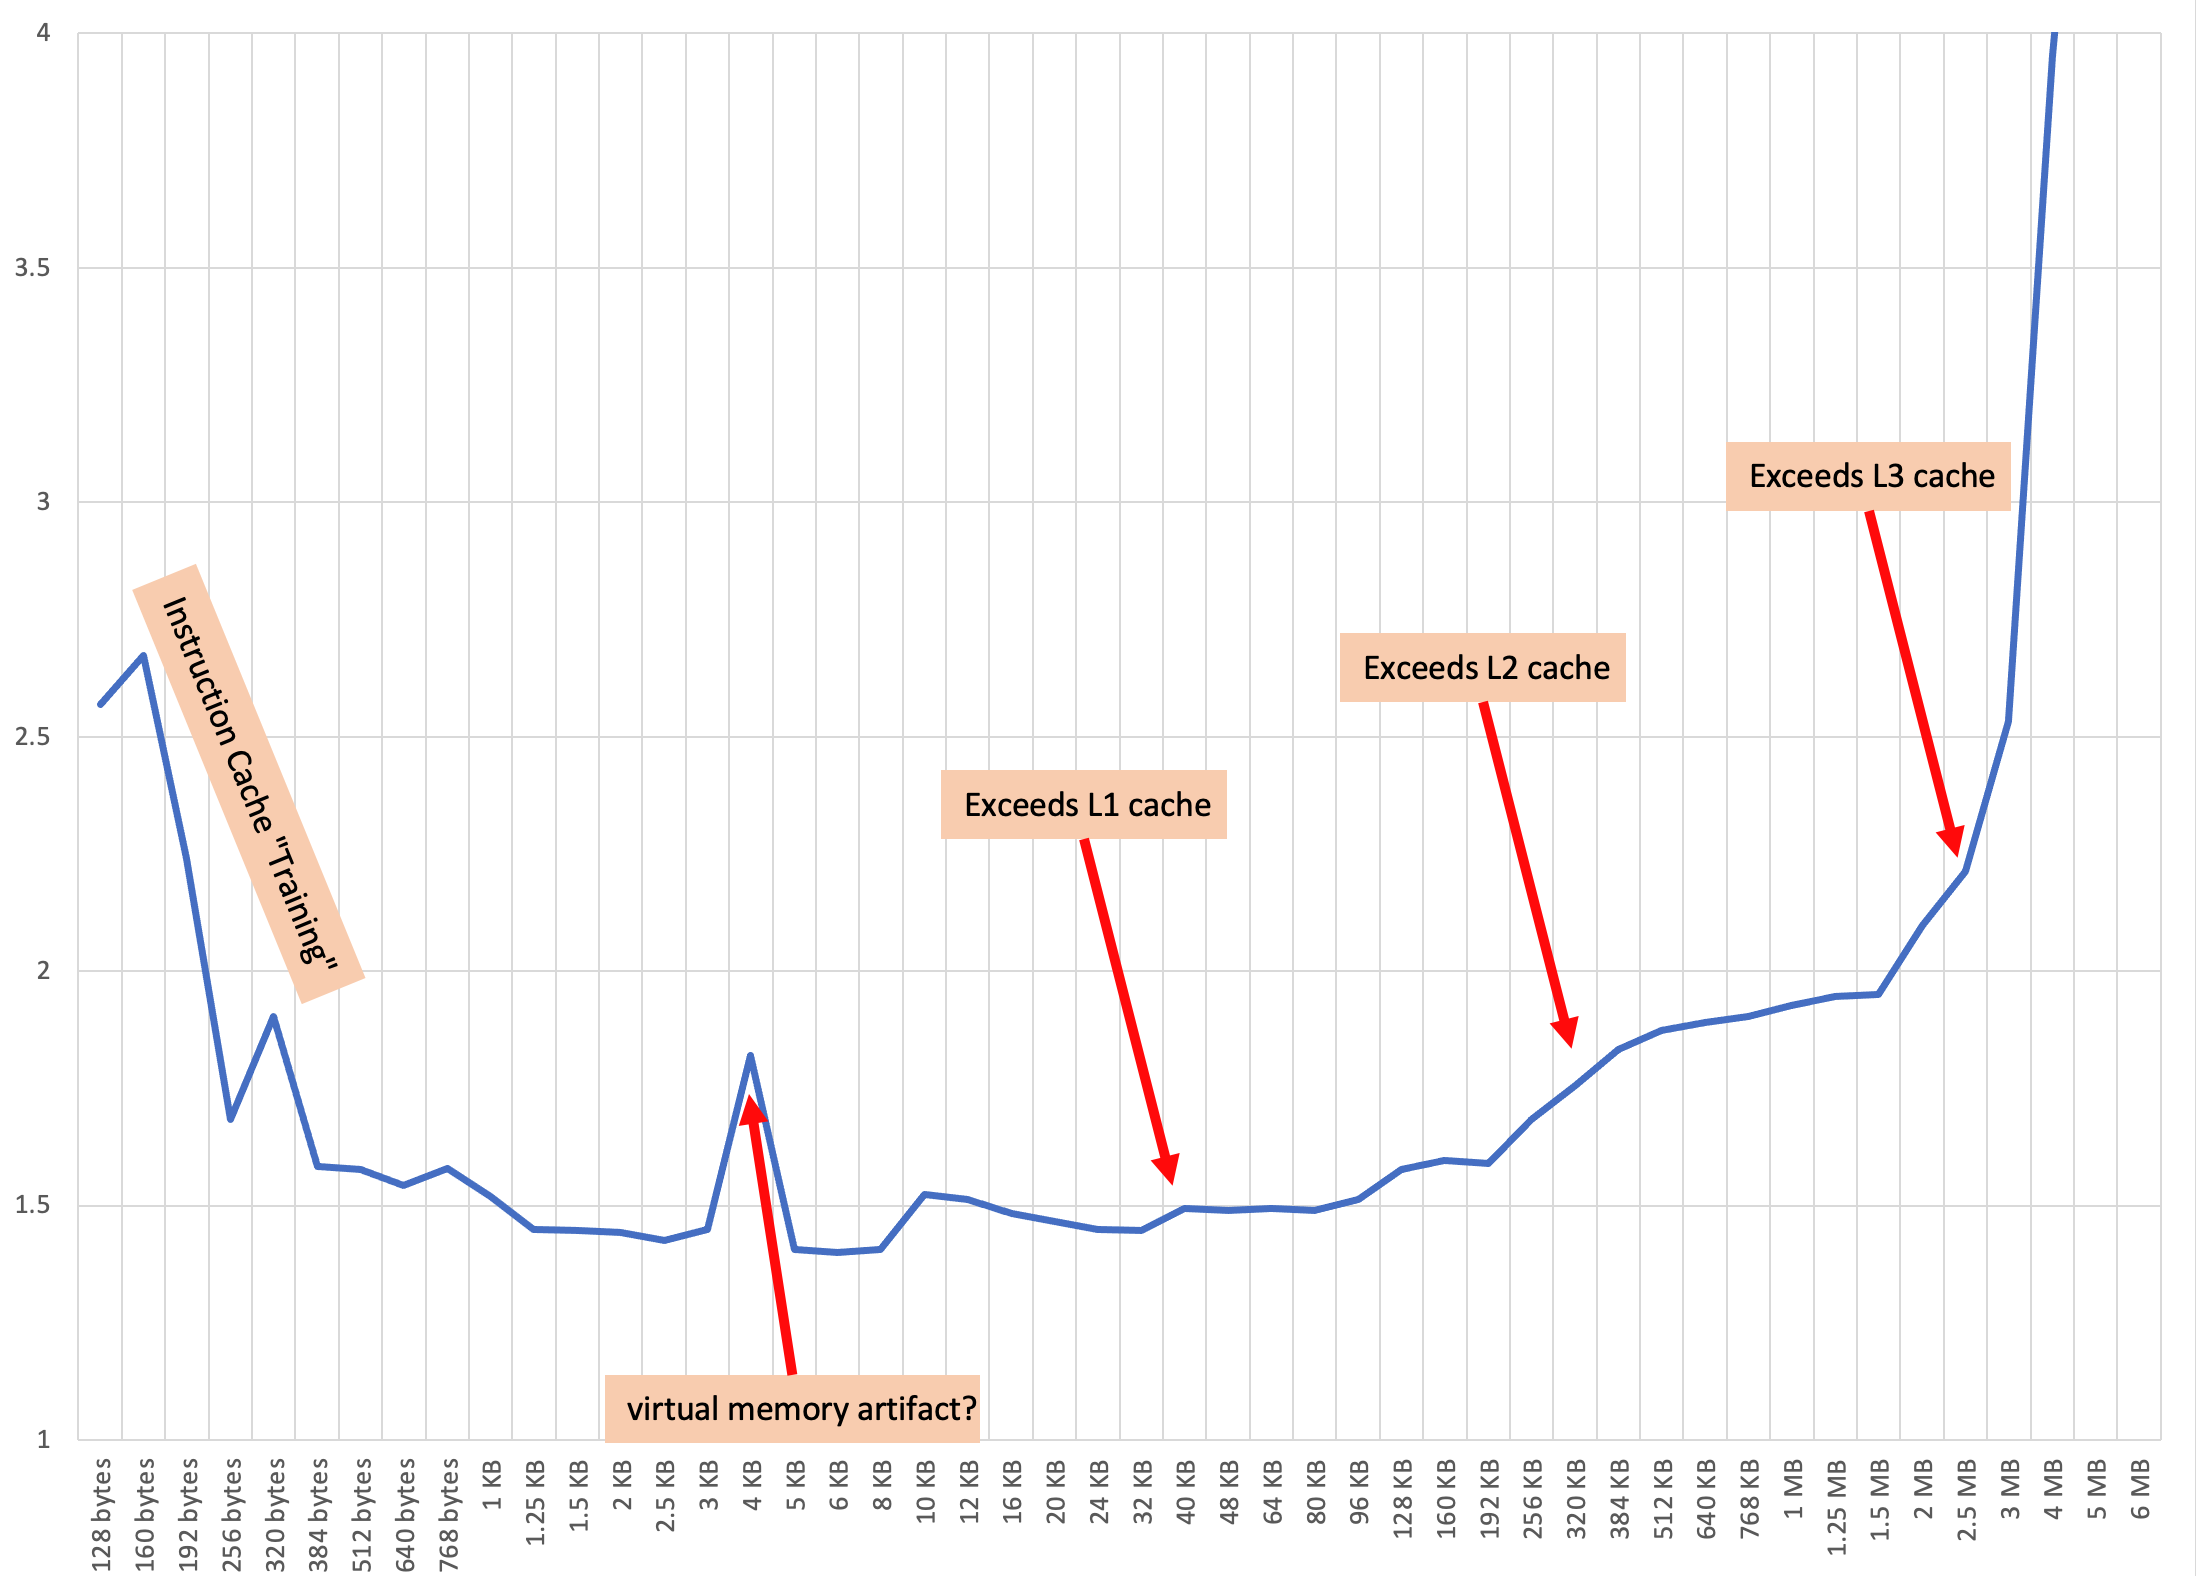
\includegraphics[width=13cm]{IntelI7caches}
    \caption{Measurement of cache levels on Intel Core i7 processor. \label{fig:LaptopCache}}
\end{figure}

The main differences between Figure~\ref{fig:LaptopCache} and the chart you'll produce are:

\begin{itemize}
    \item The RP2040 has only one cache level
    \item There is less competition for the cache on the RP2040
\end{itemize}

When taking measurements on the Intel Core i7 processor, the data can be ``mushy'' because there are other processes using the processor, which will also use the cache.
On the RP2040, the only competition for the cache will be the program's instructions which will occasionally conflict with the ``data'' we're reading,
and the occasional interrupt by MBED~OS\@.

\begin{description}
    \checkoffitem{Using your laptop's cursor in the Serial Monitor, press your laptop's \textbf{2} key (\textit{Measure the size of the instruction cache using timing data}).}
    \checkoffitem{Open the ``Raw Data'' tab in \textit{CacheCharts.xlsx} and locate the portion labeled ``CACHE SIZE by time (menu option 2)''.}
    \checkoffitem{Copy/paste the program's output from the Serial Monitor into the spreadsheet's rows 2--35.}
    \checkoffitem{Open the ``Cache Size'' tab.}
    \checkoffitem{Answer question 7 in \textit{answers.txt}.}
\end{description}

\begin{enumerate}
    \setcounter{enumi}{6}

    \item What is your estimate for the size of the RP2040's cache?

        The maximum size for which the program runs ``fast'' is the size of the cache.
\end{enumerate}


\section{Measuring the Size of a Cache Line}

One of the functions in \textit{cache\_measurement.c} is \function{measure_cache_line_by_time()}.
As with \function{measure_cache_size()}, this function iterates over an ``array'' in flash memory that can be cached.
Where \function{measure_cache_size()} held the stride constant and grew the array's size,
\function{measure_cache_line_by_time()} holds the array's size constant and grows the stride.

Recall that caches are designed to take advantage of locality, and when memory access patterns don't take advantage of locality then performance suffers.
We will exploit this fact by increasing the access stride so that you can notice when there is a slight increase in timing due to the stride exceeding the length of a cache line.
When the stride is shorter than the size of a cache line, then some accesses will be cache misses, but those misses will bring a new block into the cache.
Subsequent accesses to the same block will be cache hits.
When the stride is equal to (or greater than) the size of a cache line, then each access will be in a different block,
and every access will be a cache miss.

Figure~\ref{fig:LaptopCacheLine} shows a graph similar to the one you will produce.
The time measured by the program holds more-or-less steady up through strides of 32 bytes.
When the stride reaches 64 bytes, there is a noticeable increase in the measured time.
From this, we can conclude that the Intel Core i7's cache line is 64 bytes.

\begin{figure}
    \centering
    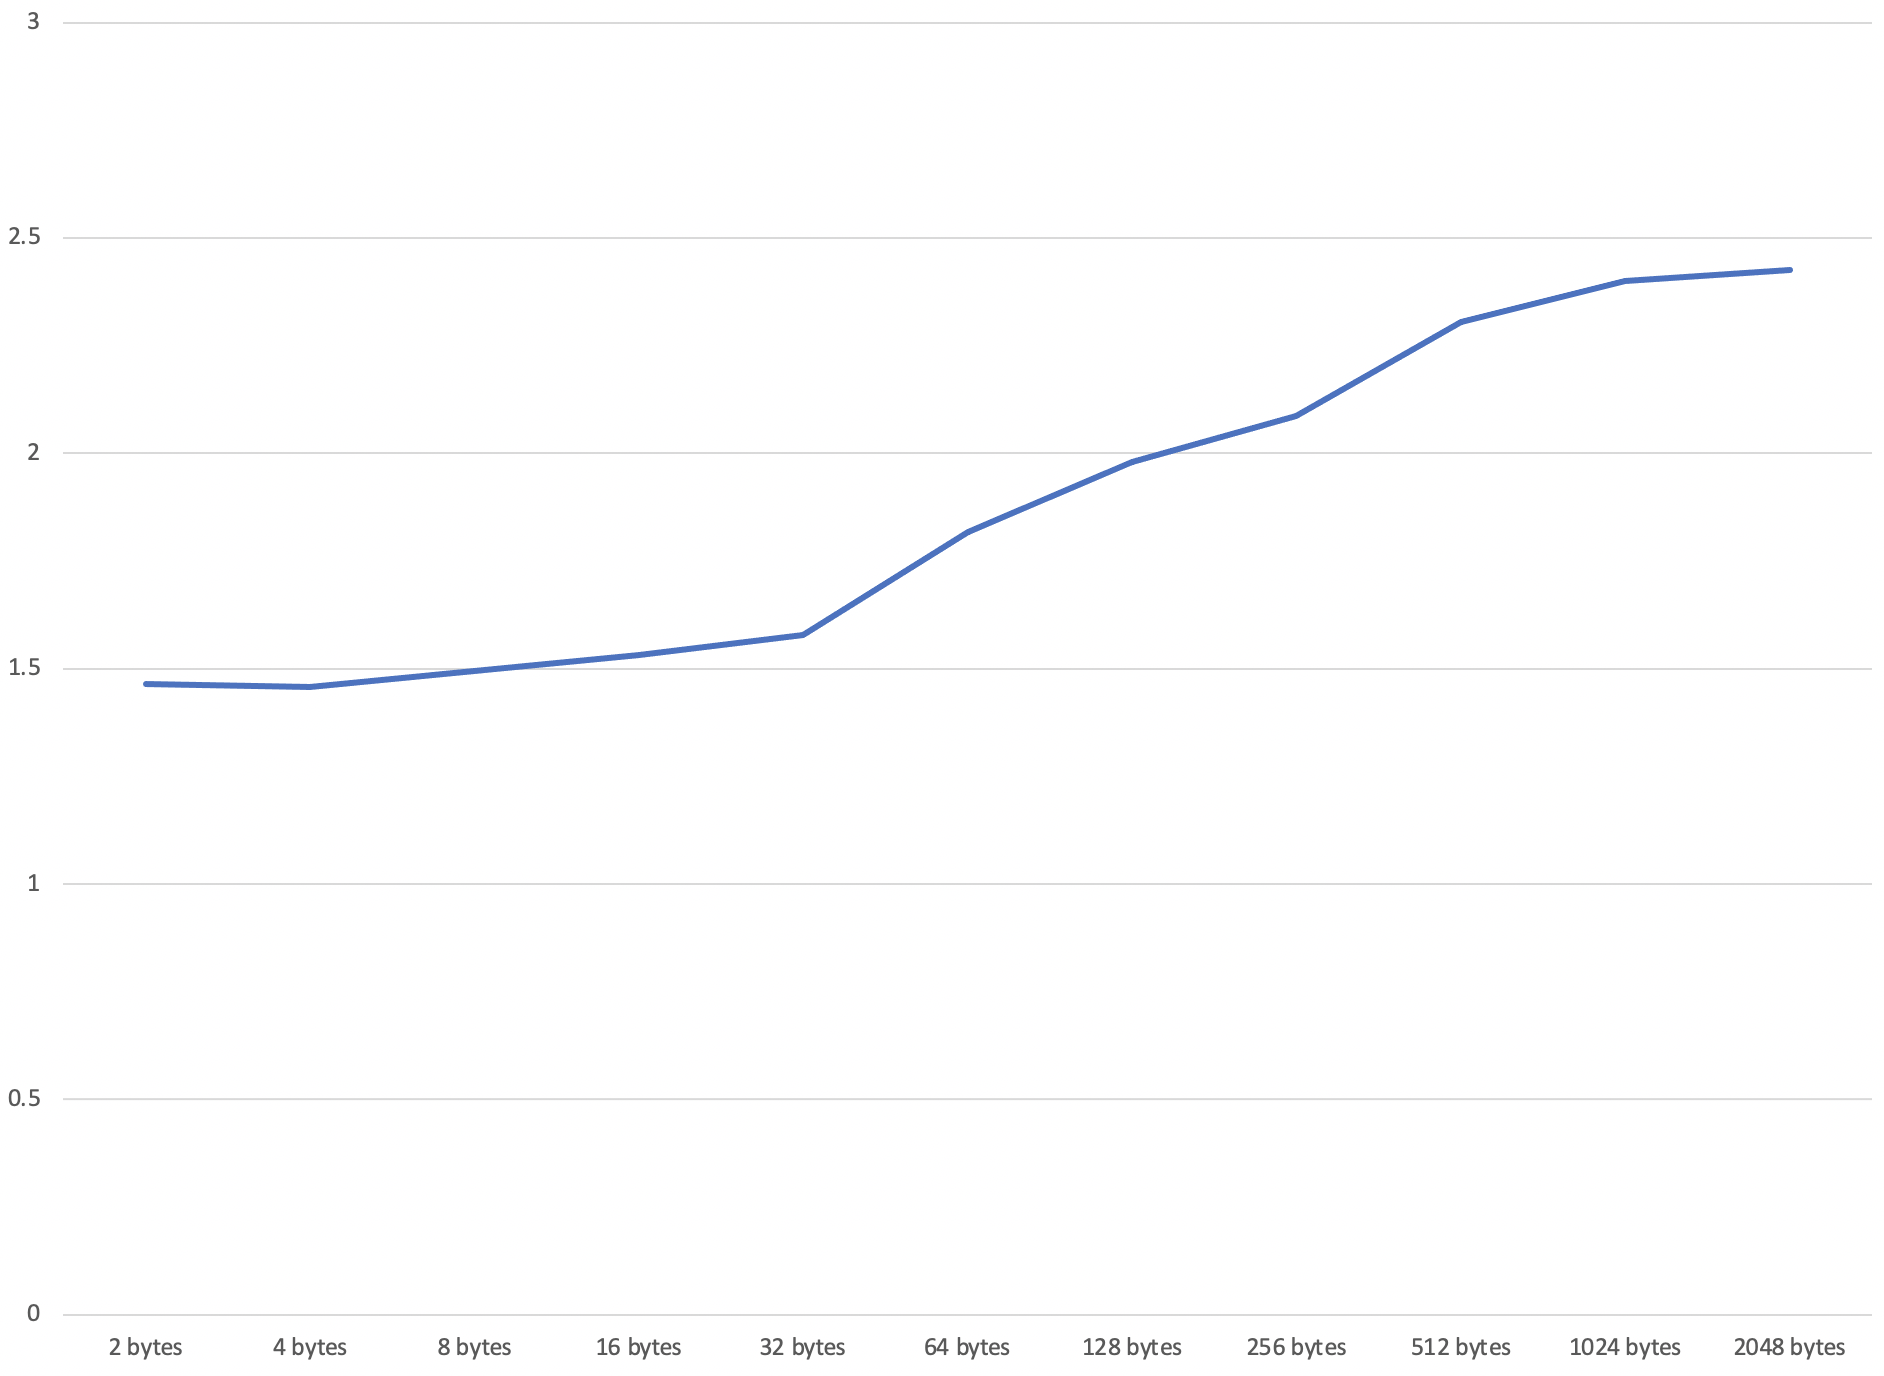
\includegraphics[width=13cm]{IntelI7cacheLine}
    \caption{Measurement of cache lines on Intel Core i7 processor. \label{fig:LaptopCacheLine}}
\end{figure}

As with the earlier cache measurement, you might see some interference from MBED~OS;
if the data doesn't seem to make sense, feel free to re-run the test.

\begin{description}
    \checkoffitem{Using your laptop's cursor in the Serial Monitor, press your laptop's \textbf{3} key (\textit{Measure the size of a cache line using timing data}).}
    \checkoffitem{Open the ``Raw Data'' tab in \textit{CacheCharts.xlsx} and locate the portion labeled ``CACHE LINE SIZE by time (menu option 3)''.}
    \checkoffitem{Copy/paste the program's output from the Serial Monitor into the spreadsheet's rows 40--45.}
    \checkoffitem{Open the ``Cache Line Size infer by time'' tab.}
    \checkoffitem{Answer question 8 in \textit{answers.txt}.}
\end{description}

\begin{enumerate}
    \setcounter{enumi}{7}

    \item What is your estimate for the size of a cache line in the RP2040's cache?

    The size at which there is a noticeable increase in time is the size of a cache line.
\end{enumerate}



\section*{Turn-in and Grading}

When you have completed this assignment, upload \textit{answers.txt} and
\textit{CacheCharts.xlsx} to \filesubmission.

This assignment is worth 10 points. \\

\begin{description}
\rubricitem{1}{Measuring the speed of SRAM and flash memory on the RP2040.}
\rubricitem{2}{Concluding whether or not the time to access data in SRAM is consistent with the Cortex-M0+ Technical Reference Manual,
    and justifying your conclusion.}
\rubricitem{2}{Drawing a reasonable conclusion about the speed of flash memory relative to the speed of SRAM.}
\rubricitem{1}{Measuring the cache size and the cache line size on the RP2040.}
\rubricitem{2}{Drawing a reasonable conclusion about the size of the RP2040's cache.}
\rubricitem{2}{Drawing a reasonable conclusion about the size of the RP2040's cache line.}
\end{description}

Your conclusions do not need to be correct to receive full credit.
You can receive full credit if your conclusions are reasonable, given your measurements.


\section*{Epilogue}

{\large \textbf{Post-Credits Scene}:} As an opportunity to stretch your legs,
you decided to walk from your office at the Pleistocene Petting Zoo to Eclectic
Electronics, to personally give Herb your memory measurement data. As you
approach Eclectic Electronics' labs, you notice that the lights are flickering,
and sparks are dripping from the ceiling. You see that a new Cow Pi-based
electronic lock is still holding the lab door shut squarely in its frame -- but
the door frame has been torn from the wall and is laying askew in the hallway.
On the floor is a Cow Pi-based calculator; the display reads: \\
\begin{tabular}{>{\raggedleft}p{3.5cm}>{\raggedleft\arraybackslash}p{1cm}}
    \rowcolor{LightGreen}\texttt{Robot Count:\phantom{xxxx}} & \texttt{12} \\
    \rowcolor{LightGreen}\texttt{-} & \texttt{1}
\end{tabular}


Peeking into the lab, you see a platform, empty except for a note. The note says:

\begin{center}\StickyNote[5cm]{\begin{center}
i\textsc{Suck \\ Robot Vacuum Cleaner \\ \phantom{x}}
\end{center}\begin{flushleft}
CAUTION! Stuck in ``Malevolent Sentience'' mode. \\ \phantom{x} \\
Do \underline{\underline{not}} turn on until after
troubleshooting the problem and uploading new software.
\end{flushleft}}[7cm]\end{center}

A Cow-Pi based motion alarm chirps as something enters its detection range.

\textit{Cut to black.}

\end{document}
